\documentclass[11pt]{article}
\usepackage{common}
\usepackage[usenames, dvipsnames]{color}
\usepackage{setspace}
\usepackage{booktabs}
\usepackage{multirow}
\usepackage{framed}

\title{CS207 Algorithm Analysis: Kernel Density Estimation}
\author{Gioia Domined\`o \and Nicolas Drizard \and Kendrick Lo \and Malcolm Mason Rodriguez}

\begin{document}
\maketitle{}

\pagestyle{plain}
\pagenumbering{arabic}

\section{Introduction}

Kernel Density Estimation (KDE) is a non-parametrical statistical technique that is used to estimate the probability density function (PDF) of a random variable based on a finite data sample\footnote{https://en.wikipedia.org/wiki/Kernel\_density\_estimation}.  Mathematically, we can denote the KDE of the PDF of independent and identically distributed (\textit{iid}) random variables $X=\{x_1, x_2, ..., x_n\}$ as:

\begin{equation} \label{eq:kde}
\hat{f}_h(x) = \frac{1}{n} \sum_{i=1}^n K_h(x - x_i) = \frac{1}{nh} \sum_{i=1}^n K \Big( \frac{x - x_i}{h} \Big)
\end{equation}

\noindent where $K(\cdot)$ represents the \textit{kernel} and $h$ represents the \textit{bandwidth} (i.e. a smoothing parameter). We note that $\hat{f}_h(x)$ denotes the estimated PDF at a particular point $x$, and that the entire data set $X$ is used to calculate it. \medskip

\noindent Various kernels are used in practice (e.g. Gaussian, Epanechnikov, exponential, etc.), all of which meet the criteria of being non-negative functions with mean zero that integrate to one. Similarly, different (strictly positive) values of $h$ can be chosen depending on the data set in question. Figure \ref{fig:kde_params} illustrates how the choice of these two parameters affects the shape of the estimated PDF.

\begin{figure}[h!]
\centering
\subfloat[Changing the kernel (bandwidth$=0.2$)]{\label{fig:kde_params_k}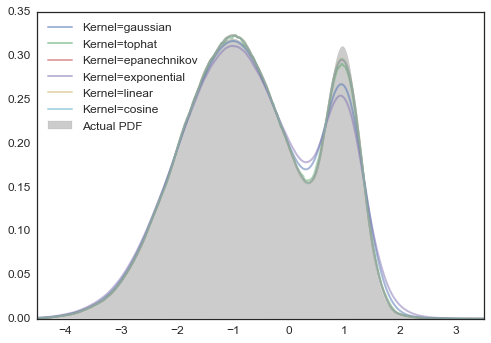
\includegraphics[width=3in]{img/change_k}}
\subfloat[Changing the bandwidth (gaussian kernel)]{\label{fig:kde_params_bw}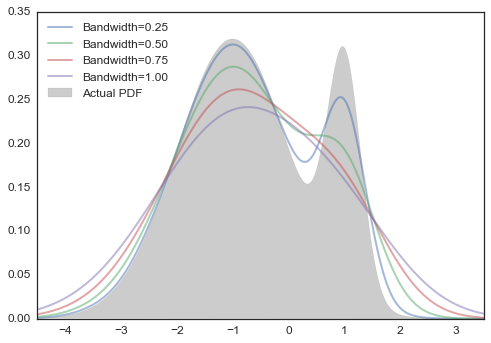
\includegraphics[width=3in]{img/change_bw}}
\caption{Impact of KDE parameters}
\label{fig:kde_params}
\end{figure}

\newpage

\section{Algorithm}

A discussion on the ``best" parameters for KDE is beyond the scope of this paper.  For ease of comparability, all our experiments are based on a Gaussian kernel and a bandwidth of $0.2$. Figure \ref{fig:sample_kde} shows the result of running the Scikit Learn KDE algorithm with these parameters on 100K one-dimensional random variables drawn from a bimodal distribution, where the PDF is plotted at 1K evenly-spaced values of $x$.

\begin{figure}[h!]
\centering
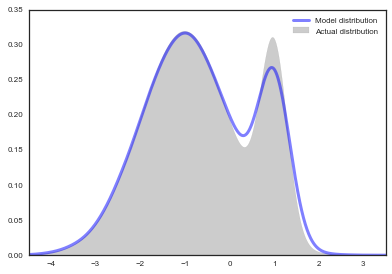
\includegraphics[width=4in]{img/sample_kde.png}
\caption{Sample KDE output}
\label{fig:sample_kde}
\end{figure}

\noindent We started by implementing a "pure" Python version of KDE (hereinafter "na\"ive KDE"); in keeping with that objective, we only used lists. We can see from the code below that the KDE algorithm is a direct application of Equation \ref{eq:kde}. The double loop, which is necessary due to the use of lists, immediately stands out as a significant source of inefficiencies.

\begin{framed}
\begin{singlespacing}
\begin{scriptsize}
\begin{verbatim}
def gaussian(x):
    '''
    Returns the Gaussian function for a given input variable.
    
    Parameters
    ----------
    x : float
        the x-value at which to evaluate the Gaussian function
        
    Returns
    ----------
    gaussian : float
        the result of evaluating the Gaussian function at x
    '''
    return np.exp(-1.0 * (x**2) / 2) * (1.0 / np.sqrt(2.0 * np.pi))
\end{verbatim}
\end{scriptsize}
\end{singlespacing}
\end{framed}

\newpage

\begin{framed}
\begin{singlespacing}
\begin{scriptsize}
\begin{verbatim}
def naive_kde(x, x_grid, h):
    '''
    Calcalates the KDE PDF estimate, based on a Gaussian kernel.
    
    Parameters
    ----------
    x : list
        iid random variables that are used to calculate the KDE estimate
    x_grid : list
        values along which to calculate the KDE estimate
    h : float
        bandwidth parameter for the KDE estimate
        
    Returns
    ----------
    estimates: list
        KDE estimates for all values of x_grid
    '''
    global N # number of iid random variables
    estimates = [0] * len(x_grid)
    
    for j, gridpt in enumerate(x_grid):
        for i in range(N):
            val_in_sum = gaussian((x[i] - gridpt) / h)
            estimates[j] += val_in_sum
        
        estimates[j] = estimates[j] / (N * h)
    
    return estimates
\end{verbatim}
\end{scriptsize}
\end{singlespacing}
\end{framed}

\noindent Before moving on to the Scikit Learn implementation, we tested the effect of switching from lists to Numpy arrays and vectorizing the inner loop. This simple change, which is shown in the code below, reduced the runtime from nearly 300 seconds to just over 1 second!

\begin{framed}
\begin{singlespacing}
\begin{scriptsize}
\begin{verbatim}
def vectorized_kde(x, x_grid, h):
    '''
    Calcalates the KDE PDF estimate, based on a Gaussian kernel.
    Inputs
    ----------
    x      : An array of iid random variables that are used to calculate the KDE estimate
    x_grid : An array of values along which to calculate the KDE estimate
    h      : Float, the bandwidth parameter for the KDE estimate
    Returns
    ----------
    An array of KDE estimates for all values of x_grid.
    '''    
    global N # number of iid random variables

    estimates = np.zeros(len(x_grid))
    
    for j, gridpt in enumerate(x_grid):
        val_in_sum = gaussian((x - gridpt)/h)  # returns vector of dim N
        estimates[j] = np.sum(val_in_sum) / (N * h)
    
    return estimates
\end{verbatim}
\end{scriptsize}
\end{singlespacing}
\end{framed}

\newpage

\section{Scikit Learn Optimizations}

After completing our Python implementation, we next moved on to examine the Scikit Learn implementation\footnote{The full source code is available at https://github.com/scikit-learn/scikit-learn/tree/master/sklearn/neighbors.} and analyze its optimizations.

%default distance metric = euclidean distance

%FFT-based computation
%For large datasets, a kernel density estimate can be computed efficiently via the convolution theorem using a fast Fourier transform. This requires binning the data, so the approach quickly becomes inefficient in higher dimensions. Of the four algorithms discussed here, only Statsmodels' KDEUnivariate implements an FFT-based KDE. As we'll see below, the FFT provides some computational gains for large numbers of points, but in most situations is not as effective as tree-based KDE implementations.


%requires homogenous datasets (vs Statsmodels' KDEMultivariate - can handle mix of  mix of continuous, ordered discrete, and unordered discrete variables)

%about a dozen distance metrics??

\begin{table}[h!]
\centering
\begin{tabular}{@{}ll@{}}
\toprule
Implementation			& Runtime (seconds)       	\\
\midrule
Na\"ive Python			& 298.28				\\
Vectorized Python		& 1.34				\\
Scikit Learn			& 5.73				\\
\bottomrule
\end{tabular}
\caption{Comparing one-dimensional KDE implementations}
\label{compare_kde}
\end{table}

\noindent
As previously noted, and as exemplified by the remarkably poor relative runtime measure above, the na\"ive or "brute force" Python KDE implementation is very slow, and it is reasonable to anticipate that its performance will lag further behind as the dimensions of the input vectors increase. The implementation requires that a distance computation be made between each input and output pair, embodied by the double loop and corresponding to a complexity of $O(n^2)$. \medskip

\noindent
Accordingly, it is not surprising that writers of alternative implementations would want to improve on the efficiency of the na\"ive algorithm. Moreover, it is clear that an algorithm of lower complexity which can implement KDE would be desirable, particularly as the problem scales. \medskip

\noindent The scikit-learn KDE implementation appears to incorporate the following optimizations:

\begin{itemize}

\item the writer provides code written in Cython; and
\item the writer utilizes \textbf{tree-based} computational methods that scale as $O(n \log n)$.

\end{itemize}

\subsection{Cython}

Cython is an extension-module generator for Python that allows code to be written in Python -- with the added requirement that type declarations be made explicit -- that can then be pre-compiled into an extension module. In this regard, Cython translates the modified Python code into a format that compiles to reasonably fast C code.  \medskip

\noindent C is a popular compiled language, and because it is compiled it is generally faster than Python. In fact, many Numpy operations are implemented in C, thus avoiding "the general cost of loops in Python, pointer indirection and per-element dynamic type checking"\footnote{see e.g. http://stackoverflow.com/questions/8385602/why-are-numpy-arrays-so-fast}. This is illustrated by the fact that our vectorized Python implementation, which is Numpy-based, is even faster than the scikit-learn implementation. For the basic KDE calculations being performed, Numpy provides significant improvement as the operations involved can be vectorized; in general, however, not all operations can be vectorized and may not lead to as significant of a performance improvement. \medskip

\noindent That said, it is important to be aware that the two implementations (scikit-learn versus Numpy) are not directly comparable since the data structures employed (and operations performed) are not identical. \medskip

\noindent In any event, despite the enhanced performance that generally comes with C implementations, C code is lower-level, which typically makes C programming slower and more cumbersome than Python programming. Therefore, the use of Cython can be seen as a reasonable compromise between performance and coding ease. \medskip

\noindent The primary Python module for the KDE implementation in scikit-learn is $kde.py$, which imports modules from .pyx files $ball\_tree$\footnote{https://github.com/scikit-learn/scikit-learn/blob/master/sklearn/neighbors/ball\_tree.pyx} and $kd\_tree$\footnote{https://github.com/scikit-learn/scikit-learn/blob/master/sklearn/neighbors/kd\_tree.pyx}, both of which are written in Cython. Additionally, the functions corresponding to different distance computations are also coded in Cython\footnote{https://github.com/scikit-learn/scikit-learn/blob/master/sklearn/neighbors/dist\_metrics.pyx}. \medskip

\noindent Finally, we also observed that some of these modules written in Cython have also been modified to support multi-threading (note the "nogil" arguments that have been incorporated into certain functions), potentially further enhancing the performance of the scikit-learn implementation.

\subsection{Tree-based Computation}

Several options for performing KDE computations in Python exist, including ones available in the SciPy and Statsmodels packages; however, according to the author\footnote{https://jakevdp.github.io/blog/2013/12/01/kernel-density-estimation/} of the scikit-learn version, none of those alternatives employ tree-based computation. The author recognized that because the na\"ive KDE algorithm requires all pairwise distance computations to be performed, KDE can be placed into "the same category as Nearest Neighbors, N-point correlation functions, and Gaussian Process Regression, all of which are examples of \textbf{Generalized N-body problems} which can be efficiently computed using specialized data structures such as a KD Tree"\footnote{Ibid.}. Importantly, these tree-based methods scale as $O(n \log n)$, making them more efficient than the $O(n^2)$ brute-force approach as $n$ gets large. How do these tree-based methods enhance performance?

\begin{quote}
The main idea is this: if you can show that a query point $Q_0$ is geometrically far from a set of training points $\{T_i\}$, then you no longer need to compute every kernel weight between $Q_0$ and the points in $\{T_i\}$: it is sufficient to compute one kernel weight at the average distance, and use that as a proxy for the others. With careful consideration of the bounds on the distances and the maximum error tolerance for the final result, it is possible to greatly reduce the number of required operations for a KDE computation.\footnote{Ibid.}
\end{quote}
 
\noindent In other words, the use of structures such as a KD Tree (a binary tree in which every node is a k-dimensional point\footnote{https://en.wikipedia.org/wiki/K-d\_tree}) or a ball tree (a binary tree in which every node defines a D-dimensional hypersphere containing a subset of the points to be searched\footnote{https://en.wikipedia.org/wiki/Ball\_tree}) effectively provide means for \textbf{approximating} the exact KDE solution. Accordingly, although performance is enhanced, there exists a tradeoff between performance and accuracy. However, the tolerances can be set in the scikit-learn implementation, where larger tolerances generally lead to faster executions. In this regard, the author asserts that even a marginal reduction in accuracy (e.g. allowing errors of 1 part in $10^8$) can lead to impressive gains in computational efficiency.


% explain why, in your opinion, the writers felt the need of an optimization
% to do this, explain the basic algorithm by writing an implementation in pure python. You can use the project's test examples to make sure your implementation is correct.
% explain the logic of the optimization

%\section{Additional Considerations}
%KDE estimation in higher-dimensional space?

\end{document}
